% TTCL @ NeurIPS 2026 workshop submission — 4–9pp main text, double-blind.
% Official NeurIPS 2026 template (submission mode: anonymized, line numbers).
% For camera-ready: \usepackage[final]{neurips_2026}.
\documentclass{article}
\usepackage[nonatbib]{neurips_2026}
% tectonic/XeTeX lacks TU-encoded ptm/phv; use OpenType Times-compatible fonts
\usepackage{fontspec}
\setmainfont{texgyretermes-regular.otf}[BoldFont=texgyretermes-bold.otf,
  ItalicFont=texgyretermes-italic.otf,BoldItalicFont=texgyretermes-bolditalic.otf]
\setsansfont{texgyreheros-regular.otf}[BoldFont=texgyreheros-bold.otf,
  ItalicFont=texgyreheros-italic.otf,BoldItalicFont=texgyreheros-bolditalic.otf]
\usepackage{amsmath,amssymb}
\usepackage[numbers,compress]{natbib}
\usepackage{booktabs}
\usepackage{pgfplots}
\pgfplotsset{compat=1.18}
\usepackage{microtype}
\usepackage[hidelinks]{hyperref}
\newcommand{\dlp}{\Delta\ell}
\title{The Write Sharpens the Query:\\ What Online In-Weight Memory Buys, and What Buys It Back}
\author{Anonymous Author(s)}

\begin{document}
\maketitle

\begin{abstract}
We stress-test online in-weight memory --- one personal fact per turn, written into a LoRA
adapter on a frozen 9B chat model at test time --- on the InMind implicit-association
benchmark, whose published external-memory systems reach at most $0.171$ of the in-context
ceiling. A pre-registered program of thirteen experiment chains moves the benchmark to
$0.53$ of that ceiling ($0.56$ of our own measured ceiling) and prices every step of the
climb, with a frozen instrument control at every step. The accounting is
deliberately unflattering to the write: an agentic retry budget subsumes the write's
keyword-level pointer gain; a genre-matched first-person question with no training anywhere
beats every trained front end we built in the isolated protocol but one; that one --- embed the adapter's
\emph{answer} to a memory-check question --- is worth a consistent but underpowered
$+0.048$ over its own frozen control; and the top pipeline ($0.448$) is the simplest of
all --- and the one place the write cashes at conventional significance: $+0.136$ over
the best frozen front end (exact $p{=}0.019$, post hoc), its gold-free controls
collapsing to $0.080$. Around this climb we measure four properties of the write
itself: a \emph{certification--retrieval dose wall} --- a membership-style likelihood
certificate turns positive at ${\sim}2$ gradient steps, while generative recall and
likelihood-scan retrieval (ranking store lines by the write-induced likelihood shift) need
${\sim}6$; a \emph{form lock with a retroactive unlock} --- a freshly written fact answers
only its trained question form until subsequent unrelated writes anneal it open, an
ordering deployment provides for free; a \emph{write-format key} --- verbatim writes key
the index to the exact string, and paraphrase writes invert the key ($0.600$ on held-out
paraphrases, $0.184$ on the original string); and a \emph{content axis of forgetting} ---
under a matched write template, burial that leaves natural facts at $0.92$--$0.95$
collapses pseudoword facts to $0.15$ strict recall, yet every likelihood certificate survives with rising
margins, and the corrupted emissions are syllable-level chimeras of competing values,
$97\%$ novel strings. The operating rules for test-time continual learning follow: serve
cold, write hot; write paraphrases if you want a meaning-keyed index; and never let a fact
be the last thing written before it is needed.
\end{abstract}

\section{Introduction}

Test-time continual learning proposals routinely measure whether a model \emph{can still
learn}; they rarely measure whether what it learned can still be \emph{read out}, and almost
never price the readout against the strongest training-free alternative. This paper is that
pricing exercise, run adversarially against our own system.

The substrate is the simplest deployable form of test-time learning: a frozen
instruction-tuned 9B chat model, a rank-64 LoRA adapter, one personal fact per turn written
by gradient descent at test time, and an append-only text log that keeps everything. The
stress test is InMind \citep{inmind2026}, an implicit-association benchmark: each of 125
tasks pairs a personal disclosure (``I have a tree-nut allergy'') with a semantically
distant application query (``walk me through a macaron recipe'') whose correct answer must
apply the fact unprompted. Published external-memory systems (Mem0, A-Mem, HippoRAG~2,
MemoryOS, xMemory, A-RAG) reach $\le 14.4\%$ indirect application against an in-context
ceiling of $84\%$ --- a relative wall of $0.171$. To our knowledge ours is the first
parametric-memory arm on this benchmark.

Two design commitments distinguish the program from a leaderboard entry. First, every arm
ships with an \emph{instrument control}: the identical pipeline with the write removed, so
each gain is attributed to memory or machinery before it is celebrated (the final
real-stream arm carries two). Second, every chain is pre-registered in a ledger with falsification lines;
the probe amendments the program needed are declared as amendments, and three instruments
that returned flattering artifacts (a retrieval probe credited by lexical overlap with the
probe itself, a membership-confounded scan, a recall criterion satisfied by echoing the
attribute word alone) were voided by our own audits before any number was kept.

\textbf{Contributions.} (1) A measured climb of a published wall from $0.171$ to $0.53$ of
the in-context ceiling ($0.448/0.84$ published; $0.56$ of the $0.80$ in-context ceiling
we measure on our own backbone and judge), with
the attribution honestly split between instrument and memory at every step
(\S\ref{sec:climb}). (2) The certification--retrieval dose wall: recognition-style
certification and retrieval-usable storage separate by ${\sim}3\times$ in write dose, on
both the generative and the discriminative readout (\S\ref{sec:wall}). (3) The write-format
key: what surface family the writes exercise determines --- bidirectionally --- what the
memory index retrieves by (\S\ref{sec:key}). (4) A content axis that reconciles
``catastrophic forgetting within a handful of writes'' with ``nothing forgets'': under a matched harness,
interference-robustness is a property of the content's pretraining
prior, and what interference corrupts is the emission sequence, not the discrimination
trace (\S\ref{sec:content}).

\section{Setup}\label{sec:setup}

\textbf{Protocol.} We follow the benchmark's canonical per-task isolation: memory state = a
47-session background corpus (240 user turns indexed) plus one injected fact, a 241-line
store per task. Writes are teacher-forced gradient steps on the fact (a \texttt{Note} form
and a chat-QA form against the task's direct question, prefix-masked), $3{\times}10^{-5}$,
rank-64 all-linear LoRA. Two per-fact doses recur throughout, named by the readout tier they
reach: the \emph{certification dose} (${\sim}2$ steps, at which a calibrated likelihood
certificate turns positive) and the \emph{recall dose} (${\sim}6$--$8$ steps, at which the
persona-prompted direct question --- the model told it may know the user personally ---
is answered from weights). Serving is always cold: the
frozen base generates every user-facing answer from retrieved log lines. Two recurring
terms: a line's \emph{register} is its surface voice (the store's lines are first-person
conversational); the write's \emph{pointer} is a keyword elicited from the adapter and
used to seed retrieval.

\textbf{Instruments.} Retrieval is scored as gold-in-top-$k$, $k{=}6$ (agentic arms
credit gold in any round's top five), over the 241-line store
(BGE-small embeddings; prefixing the encoder's retrieval instruction to the query arm
leaves its scores unchanged --- $0.016$/$0.024$ at $k{=}4$/$6$ either way on the weakest
probe --- so that weakness is semantic, not an encoder artifact). End-to-end scores use the benchmark's
own application rubric verbatim, judged by a strong external model in four independent
shards; judge noise is anchored at one verdict flip per 90 byte-identical answers. The
discriminative readout is $\dlp$: mean per-token log-probability shift of a candidate line,
adapter versus pre-write base --- a reference-calibrated membership statistic
\citep{carlini2022lira,duan2024mia} repurposed as a read head, and never treated as recall:
the gap between the index and what can be emitted is the object of study
\citep{song2026beyondppl}. All arms return few, precise lines: application of a
retrieved fact decays monotonically in context size once coverage is conditioned away
\citep{jin2025longrag,cuconasu2024noise}.

\section{The climb, priced}\label{sec:climb}

\begin{figure}[t]
\centering
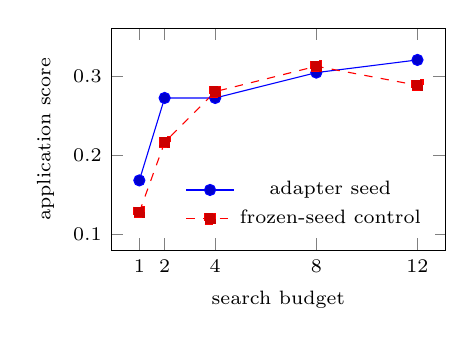
\begin{tikzpicture}
\begin{axis}[width=0.48\linewidth,height=4.4cm,
  xlabel={search budget},ylabel={application score},
  xtick={1,2,4,8,12},ymin=0.08,ymax=0.36,
  legend style={at={(0.97,0.05)},anchor=south east,font=\scriptsize,draw=none},
  label style={font=\scriptsize},tick label style={font=\scriptsize}]
\addplot+[mark=*] coordinates {(1,0.168)(2,0.272)(4,0.272)(8,0.304)(12,0.320)};
\addlegendentry{adapter seed}
\addplot+[mark=square*,dashed] coordinates {(1,0.128)(2,0.216)(4,0.280)(8,0.312)(12,0.288)};
\addlegendentry{frozen-seed control}
\end{axis}
\end{tikzpicture}\hfill
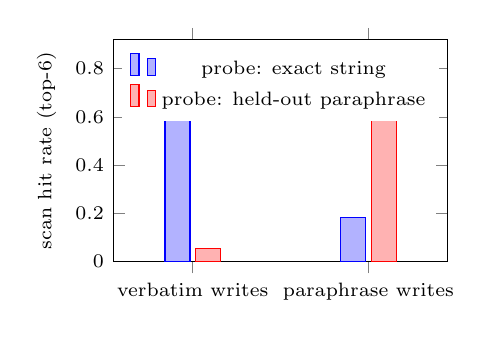
\begin{tikzpicture}
\begin{axis}[width=0.48\linewidth,height=4.4cm,ybar,bar width=9pt,
  ylabel={scan hit rate (top-6)},ymin=0,ymax=0.92,
  symbolic x coords={verbatim writes,paraphrase writes},xtick=data,
  enlarge x limits=0.45,
  legend style={at={(0.5,0.97)},anchor=north,font=\scriptsize,draw=none},
  label style={font=\scriptsize},tick label style={font=\scriptsize}]
\addplot coordinates {(verbatim writes,0.632)(paraphrase writes,0.184)};
\addlegendentry{probe: exact string}
\addplot coordinates {(verbatim writes,0.056)(paraphrase writes,0.600)};
\addlegendentry{probe: held-out paraphrase}
\end{axis}
\end{tikzpicture}
\caption{\textbf{Left:} the seeded-agentic advantage is an inverted-U in retry budget ---
$+0.056$ at budget 2, statistically zero from budget 4 on (\S\ref{sec:climb}); $n{=}125$
per point. \textbf{Right:} the write-format key inverts --- under verbatim writes the
likelihood scan retrieves the exact string and not its paraphrase; paraphrase writes flip
both bars (\S\ref{sec:key}).}
\label{fig:panels}
\end{figure}

Table~\ref{tab:ladder} compresses the program. Three attribution results discipline the
narrative before any celebration.

\begin{table}[t]
\centering\small
\begin{tabular}{llcc}
\toprule
Arm (all serve cold) & Write role & Retrieval@6 & Application \\
\midrule
Published best external system & --- & --- & $0.144$ \\
Frozen keyword front end (ours) & none & $0.152$ & $0.144$ \\
Agentic retry loop ($\le4$ searches) & none & $0.216$ & $0.176$ \\
Per-task write, keyword elicited & pointer & $0.216$ & $0.184$ \\
Seeded agentic (adapter seed) & pointer & $0.392$ & $0.272$ \\
Seeded agentic (\emph{frozen} seed control) & none & $0.360$ & $0.280$ \\
Frozen user-voice question embed & none & $0.384$ & $0.312$ \\
Adapter hop-answer embed & query gen. & $0.464$ & $0.360$ \\
\midrule
Real-stream statement embed & query gen. & $0.576$ & $\mathbf{0.448}$ \\
Real-stream controls (no writes / chatter-only) & no gold & $0.080$ & $0.080$ \\
\midrule
In-context ceiling (benchmark's backbone) & --- & --- & $0.84$ \\
\bottomrule
\end{tabular}
\caption{The canonical program. Every write arm has a frozen instrument control;
$n{=}125$ throughout; single judge (four shards). The real-stream controls run the
identical statement pipeline with the gold write removed (with or without the 51 chatter
writes --- the two collapse to byte-identical refusals), so the last step is the
write's ($+0.136$ over the best frozen front end, exact $p{=}0.019$, post hoc).}
\label{tab:ladder}
\end{table}

\textbf{The retry budget subsumes the pointer.} Seeding an agentic searcher with the
adapter's elicited keyword looks like a win ($0.272$) until the control --- the same loop
seeded with the frozen base's keyword --- scores $0.280$. The seeds agree on $92/125$ tasks;
a budget sweep over $\{1,2,4,8,12\}$ searches (Fig.~\ref{fig:panels}, left) shows the seed
advantage is an inverted-U peaking at budget 2 ($+0.056$) and statistically zero from
budget 4 on --- the seed's retrieval edge persists at every budget, but answer-side churn
over the shared hits cancels it end-to-end. The agent also self-terminates at $3.3$
searches regardless of allowance --- in this short-horizon regime the budget is not the
binding constraint, persistence is \citep{fishing2025iterative}.

\textbf{Genre beats machinery.} Embedding a generated first-person memory-check question
(``Did I tell you about\ldots?'') retrieves at $0.384$ with no training anywhere ---
register match with the log's own first-person lines, the HyDE/HyPE mechanism
\citep{gao2023hyde,vake2026hype} manufactured at query time because a per-user append-only
log cannot be question-indexed in advance. Under the isolated protocol this frozen front
end beats every trained front end we built except one.

\textbf{The write's cashable residue is a query sharpener.} The one exception (the
``hop-answer'' row): let the adapter \emph{answer} the memory-check question and embed its
answer. The write does not generate for the user; it sharpens the query with words the
frozen base cannot know ($0.464$ retrieval, $0.360$ end-to-end, $+0.048$ over the frozen
control --- consistent across the program but underpowered at $n{=}125$, one-sided sign
test $p{=}0.22$). The comparator is conservative: embedding the \emph{frozen} base's
answer to the same question collapses into refusals ($0.080$, the factorial's
frozen--frozen cell), so the question itself is the strongest frozen front end.

\textbf{Realism cashes the write.} Writing a 41-turn subset of the background stream
into the same adapter before the fact, and ten further turns after it --- the deployment
condition --- lifts the simplest pipeline (state your best guess about the user; embed
the sentence) to $0.576/0.448$; the post-fact writes are load-bearing
(\S\ref{sec:wall}). Two controls run the identical statement pipeline with the gold
write removed --- once with no writes at all, once with the 51 chatter writes but no
gold --- and both collapse to $0.080$ retrieval / $0.080$ application, every statement
the byte-identical refusal ``I don't remember'' ($125/125$ in each). The collapse
indicts only the statement form, not frozen retrieval (frozen statement $0.080$ vs
frozen question $0.384$): what it kills is the register-echo reading of this pipeline.
The two margins price different things: the isolated protocol prices the write within
its pipeline ($+0.048$, underpowered); the real stream prices it against the strongest
frozen alternative --- $+0.136$ end-to-end ($32{:}15$ discordant tasks, exact McNemar
$p{=}0.019$, computed post hoc; the pre-registered lines were the control collapses),
and $+0.368$ within the pipeline itself. The frozen maximum $0.312$ is shared by a
budget-8 frozen-seed agentic arm; the margin survives that comparator too ($35{:}18$,
$p{=}0.027$). And the edge concentrates at small $k$ (post-hoc rank curves: written
statement $0.520$ vs frozen question $0.248$ at $k{=}1$, a $2.1\times$ margin narrowing
to $1.3\times$ by $k{=}20$; the written front end at $k{=}1$ beats the frozen one at
$k{=}20$) --- the write buys precision, not recall (end-to-end application at $k{=}1$
untested).

\section{The certification--retrieval dose wall}\label{sec:wall}

The climb priced the readout; the remaining sections leave the benchmark and characterize
the write itself. Recognition-before-recall ordering is known for fine-tuned memories
\citep{orhan2023recognition}; the program puts it on a controlled dose axis, on two readout
mechanisms at once. At the certification dose the $\dlp$ certificate is positive
($125/125$ across the program) --- and nothing else works. The certificate is not a
curiosity of this rig: in the companion program (anonymized supplementary) the same
adapter-versus-base signal separates written from never-written content at AUC
$0.93$--$0.99$ with the pre-write base at chance by construction, and recognition
survives recall death across mechanisms --- a matched-budget editing arm recalls
$0$--$1/48$ while recognizing $45$--$47/48$. The generative route is dead in
every cell of a $2{\times}2$ probe factorial (who generates the memory-check question
$\times$ who answers it, frozen base or adapter). The discriminative route fails more
instructively: under a realistic write stream, scanning the store by $\dlp$ at the
certification dose ranks the just-written fact near the \emph{bottom} ($236/241$ median),
because register spillover from the other writes lifts every same-register line ---
written or not --- above the two-step needle. At the recall dose both routes open
(generative statement $0.576$; verbatim scan $0.640$, median rank 2). There is no cheap
discriminative shortcut: certification and retrieval are separated by a ${\sim}3\times$
dose wall, and below it the index is not weak but \emph{actively wrong}.

\textbf{Form lock and the retroactive unlock.} Between the doses sits an access pathology.
A fact written to the recall criterion answers its trained question form and nothing else:
off-form prompts (``state what you remember'') fall into the learned-default refusal
\citep{kang2024unfamiliar}; re-voicing the probe \emph{as the user would ask it} unlocks
genuine recall from $3.2\%$ to $32.8\%$ (this is not the reversal curse
\citep{berglund2024reversal}: argument order never changes, only the speech-act register).
The lock is released for free by deployment itself: probed immediately after its writes a
fact is locked regardless of what preceded them; a few \emph{subsequent} unrelated writes
anneal it open ($0.136 \to 0.576$ retrieval; refusals $0.71 \to 0.12$). Mixing diverse data
to unlock extraction is established offline
\citep{allenzhu2024,chen2024remix,sun2025mixed,wu2026rote}; the retroactive release of an
\emph{earlier} locked fact by \emph{later} unrelated writes --- the ordering a live
conversation supplies automatically --- is the part we have not found stated. The
scheduling rule follows: a fact should not be the last thing written before it is needed.

\section{The write-format key}\label{sec:key}

What is the index keyed on? Under verbatim writes, the recall-dose scan retrieves the exact
string ($0.632$; the independent dose-wall run of \S\ref{sec:wall} replicates at
$0.640$) and nothing else: a held-out paraphrase scores $0.056$
(Fig.~\ref{fig:panels}, right). Writing a fresh
paraphrase each round \emph{inverts} the key: the held-out paraphrase rises to $0.600$
while the original string --- still trained, via the chat-QA form --- falls to $0.184$.
A family-level control separates content from style: under paraphrase writes, the held-out
paraphrase of the \emph{written} fact gains $\dlp = 1.77$ while style-matched paraphrases
of five \emph{other, never-written} facts --- same generator, same register --- gain only
$0.09$; the content lift ($1.68$) is positive on $125/125$ tasks. The key is on the
meaning, not the style. A reversal probe on the same adapters closes the taxonomy: forward
recall passes $123/125$, yet asking the value-to-attribute direction succeeds on only
$0.08$--$0.16$ --- the register axis (unlockable, \S\ref{sec:wall}) and the argument-order
axis \citep{berglund2024reversal} coexist and dissociate on the same facts. Augmentation-enables-extraction
is the Physics-of-LMs result \citep{allenzhu2024}; the bidirectional inversion, read off a
held-out-surface likelihood index rather than QA accuracy, upgrades ``write format gates
extraction'' to ``write format \emph{selects the key}.'' For a deployed index the
consequence is directly actionable: write paraphrases, not transcripts, if you want the
memory keyed on meaning.

\section{The content axis, and what interference corrupts}\label{sec:content}

Forty subsequent one-step chatter writes kill nothing above an eight-step
\emph{natural-language} fact: recall $0.92$--$0.95$ at $n{=}125$ across both write
regimes, certificates $1.00$ with rising margins (an $n{=}8$ smoke test with
same-register fact burial replicates the survival). Rerunning the write-and-burial harness with unguessable
pseudoword facts (``My transit code is roptavvor''; burial now same-register pseudoword
writes) collapses recall to $0.15$ (strict value production) --- while every certificate survives, margins \emph{rising} from $3.8$ to
$5.2$ nats through the burial, and the scan still returns the fact in the top six.
Retention under sequential writes is known to depend on presentation breadth
\citep{oneill2026continual} and dataset provenance \citep{chen2024remix}; the axis isolated
here is \emph{lexical/entity familiarity} under a matched write template ---
distinct from propositional prior-conflict, where the sign can invert
\citep{oneill2026continual} --- and it is large enough to reconcile the pseudoword-stream
and natural-fact literatures: both are right, about different content.

The failures say what interference does. Of 125 burial tasks, 67 strict-recall failures
still emit a pseudoword-shaped value; $97\%$ of these are \emph{chimeras} --- novel strings
equal to neither the true value nor any competitor --- with own-syllable retention $0.318$
against a $0.144$ random-draw expectation ($2.2\times$) and first-syllable retention
$2.7\times$ chance. Interference under continued writing is not erasure and not
substitution: it is structure-preserving recombination of the emission sequence, carrying
above-chance target content, while the discrimination trace strengthens. Accuracy-only
metrics are structurally unable to see this; a likelihood read head plus nonsense content
makes it visible.

\section{Operating rules, and limits}\label{sec:rules}

For test-time continual learning systems the program compresses to five rules. (1)
\emph{Serve cold, write hot}: every end-to-end gain lived on the query side --- what the
weights know helps only by changing what is retrieved into context. No cold-serving arm
here loses to a hot one, and the companion program (anonymized supplementary) prices the
hot path below zero: as a reader of identical retrieved lines the adapter \emph{loses} to
the frozen base ($0.136$ vs $0.216$ application), and a consolidation policy that
rehearses the model's own outputs retains $4.3$ of $144$ facts where doing nothing
retains $25.0$ --- serving cold is load-bearing, not stylistic.
(2) \emph{The index is a query sharpener}: its cashable value is answering the system's own
memory-check question with words the frozen model cannot know. The keyword-level pointer
is priced at zero once an agentic loop may re-query (whether the sharpener itself survives
an agentic reader is untested), so it matters most where latency or search budgets bind ---
and there the edge is largest ($2.1\times$ at $k{=}1$, \S\ref{sec:climb}): the write
buys precision, not recall. (3) \emph{Certification is not retrieval}: a membership-style
certificate at two steps proves presence, not findability; budget the recall dose if the
weights must be searched. A continual stream need not pay that dose per turn: in the
companion program, dose buys acquisition speed, not end-state capacity (recognition
pinned at ${\approx}0.5$ of the stream across an $8\times$ dose and $30\times$
learning-rate sweep), and the deployed policy --- one step per turn plus miss-gated
replay (re-writing only what a self-test missed), which reaches the recall dose
\emph{across} turns --- maintains a 384-fact stream
at $0.815$--$0.849$ recall (three seeds) on this same 9B substrate with an $O(1)$
per-turn budget. (4) \emph{The write format chooses the key}; paraphrase writes
buy a meaning-keyed index at the cost of the verbatim key. (5) \emph{Schedule writes so no
fact is freshest at query time}; deployment usually does this for free.

\textbf{Limits.} One benchmark, one 9B substrate, one embedder, single external judge
(noise anchored at $1/90$); the published-system baselines are quoted, not rerun --- the
frozen keyword front end's exact tie with the published best ($0.144$) is the one
cross-rig calibration point; the $+0.048$ margin is a consistent direction, not a finding;
the real-stream register assist is attributed only jointly (chatter-only writes produce
pure refusals, so register-learning cannot be isolated from the fact write on this
probe); the content axis is demonstrated under one fixed harness (write form and
criterion were not separately varied); and the $0.53$ headline is measured on natural
personal facts against the benchmark's published ceiling --- it does not transfer across
content classes, judges, or backbones. All runs use a single consumer GPU; full per-chain
pre-registrations, amendment history, raw timelines, exact configs, and the voided
instruments ship with the anonymized artifact bundle in the supplementary material.

\section*{AI assistance disclosure}
This paper's experiments, drafts, and audits were produced with substantial AI assistance
(Claude, Anthropic) under the authors' direction; all pre-registrations, results, and the
decision to void or keep every instrument were reviewed by the human author, who bears
responsibility for the claims.

\bibliographystyle{plainnat}
\bibliography{merged}

\end{document}
